\setAuthor{Aigar Vaigu}
\setRound{piirkonnavoor}
\setYear{2017}
\setNumber{G 4}
\setDifficulty{2}
\setTopic{Geomeetriline optika}

\prob{Piiritusetehas}
Piiritusetehases mõõdetakse piirituse ja vee segus oleva piirituse mahuprotsenti joonisel näidatud optilise seadme abil, kus segu paikneb kanalis laiusega $d=\SI{1}{cm}$. 
Kui suure vahemaa võrra muutub seadme fototundlikul elemendil kiire asukoht, kui piiritus mahuprotsendiga \SI{40}{\percent} asendada piiritusega mahuprotsendiga \SI{85}{\percent}?
Võib eeldada, et segu murdumisnäitaja $n\idx{segu}$ on lineaarne kombinatsioon vee ja piirituse murdumisnäitajatest
$$
n\idx{segu}=Xn\idx{piiritus}+(1-X)n\idx{vesi},
$$
kus X on piirituse mahuline sisaldus vahemikus 0 -- 1 ja $n\idx{piiritus}=\num{1,3615}$ ning $n\idx{vesi}=\num{1,3330}$.

\begin{center}
	\vspace{-0pt}
	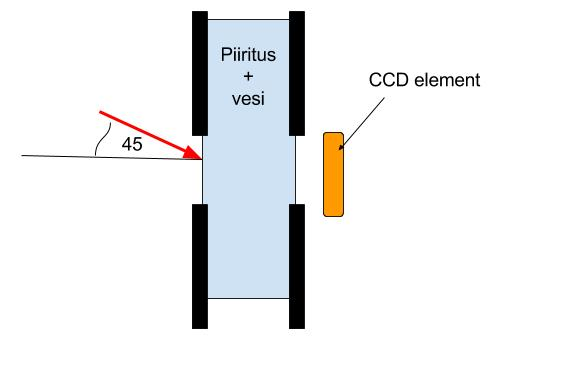
\includegraphics[width=0.5\linewidth]{2017-v2g-04-Piiritusetehas.jpg}
	\vspace{-10pt}
\end{center}

\hint
Ainus muutus kiire teekonnas toimub segu sees. Murdumisnäitaja muutuse tõttu hakkab kiir segus teise nurga all liikuma. Vastavat nurga muutust ning seejärel ka $y$-suunalist nihet on võimalik leida Snelli seaduse abil.

\solu
Murdumisseaduse järgi kehtib valguse murdumisel
$$n_0\sin(\alpha_0)=n_1\sin(\alpha_1),$$
kus $n_0$ ja $n_1$ on vastavalt esimese ja teise keskkkonna murdumisnäitajad ning $\alpha_0$ ja $\alpha_1$ on vastavalt langemis- ja murdumisnurk. Seda valemit saab iteratiivselt jätkata järgmise murdumise jaoks kolmanda keskkonna piiril, kui keskkonnad on paralleelsete kihtidena:
$$n_0\sin(\alpha_0)=n_1\sin(\alpha_1)=n_2\sin(\alpha_2) = \dots$$
Selle abil näeme, et kehtib $\sin(\alpha_j)=\frac{n_0}{n_j}\sin(\alpha_0)$. See tähendab seda, et kiire murdumisnurk sõltub ainult hetke keskkonna murdumisnäitajast ja mitte sellest, kas ja kui mitu erinevat kihti varasemalt on läbitud. Seetõttu saame ignoreerida kanalit ümbritsevat klaasist või muust materjalist kihti, arvutamaks kiire nurka kanalis. Samuti, kuna ainult piirituse ja vee segu murdumisnäitaja muutub, siis ainult kanalis on kiirte liikumisnurgad erinevad. Mujal on kiire liikumine täpselt sama, ainult pärast segu läbimist on kiir nihutatud, kui segu murdumisnäitajat muuta. Segus kehtib:
$$\sin(\alpha_{\text{segu}})=\frac{n_0}{n_{\text{segu}}}\sin{\alpha_0} = \frac{1}{\sqrt{2}n_{\text{segu}}},$$
kus $\sin(\alpha_0) = 1/\sqrt{2}$ ja õhus $n_0=1$. Kiire nihe kanali sees piki kanali suunda on lihtsa geomeetria abil $$y=d\tan(\alpha_{\text{segu}}).$$
Kasutades seost $\tan(\phi) = \frac{\sin(\phi)}{\cos(\phi)} = \frac{\sin(\phi)}{\sqrt{1-\sin(\phi)^2}}$ saame
$$y = d \frac{\sin(\alpha_{\text{segu}})}{\sqrt{1-\sin(\alpha_{\text{segu}})^2}} = \frac{d}{\sqrt{2}\sqrt{n_{\text{segu}}^2-\frac12}}.$$
Nüüd leiame $y$ kahel juhul, kui $X=\num{0.40}$ siis $y=\SI{6.184}{\milli\meter}$ ja kui $X=\num{0.85}$ siis $y=\SI{6.104}{\milli\meter}$. Saame $y$ erinevuseks
$$|\Delta y| \approx \SI{80}{\micro\meter}.$$

\probeng{Ethanol factory}
In an ethanol factory, with the help of the optical device shown in the figure, the volume percentage of ethanol is measured in a spirit and water mixture. The mixture is located in a canal of width $d=\SI{1}{cm}$. By what distance does the location of the ray on the device's photosensitive element change if the ethanol with a volume percentage 40 \% is replaced by an ethanol with a volume percentage 85 \%? You can assume that the refractive index $n\idx{mix}$ of the mixture is a linear combination of the refractive indexes of water and spirit
$$
n\idx{mix}=Xn\idx{ethanol}+(1-X)n\idx{water},
$$
where X is ethanol’s volume content ranging from 0 to 1, $n\idx{ethanol}=\num{1,3615}$ and $n\idx{water}=\num{1,3330}$.
\begin{center}
	\vspace{-0pt}
	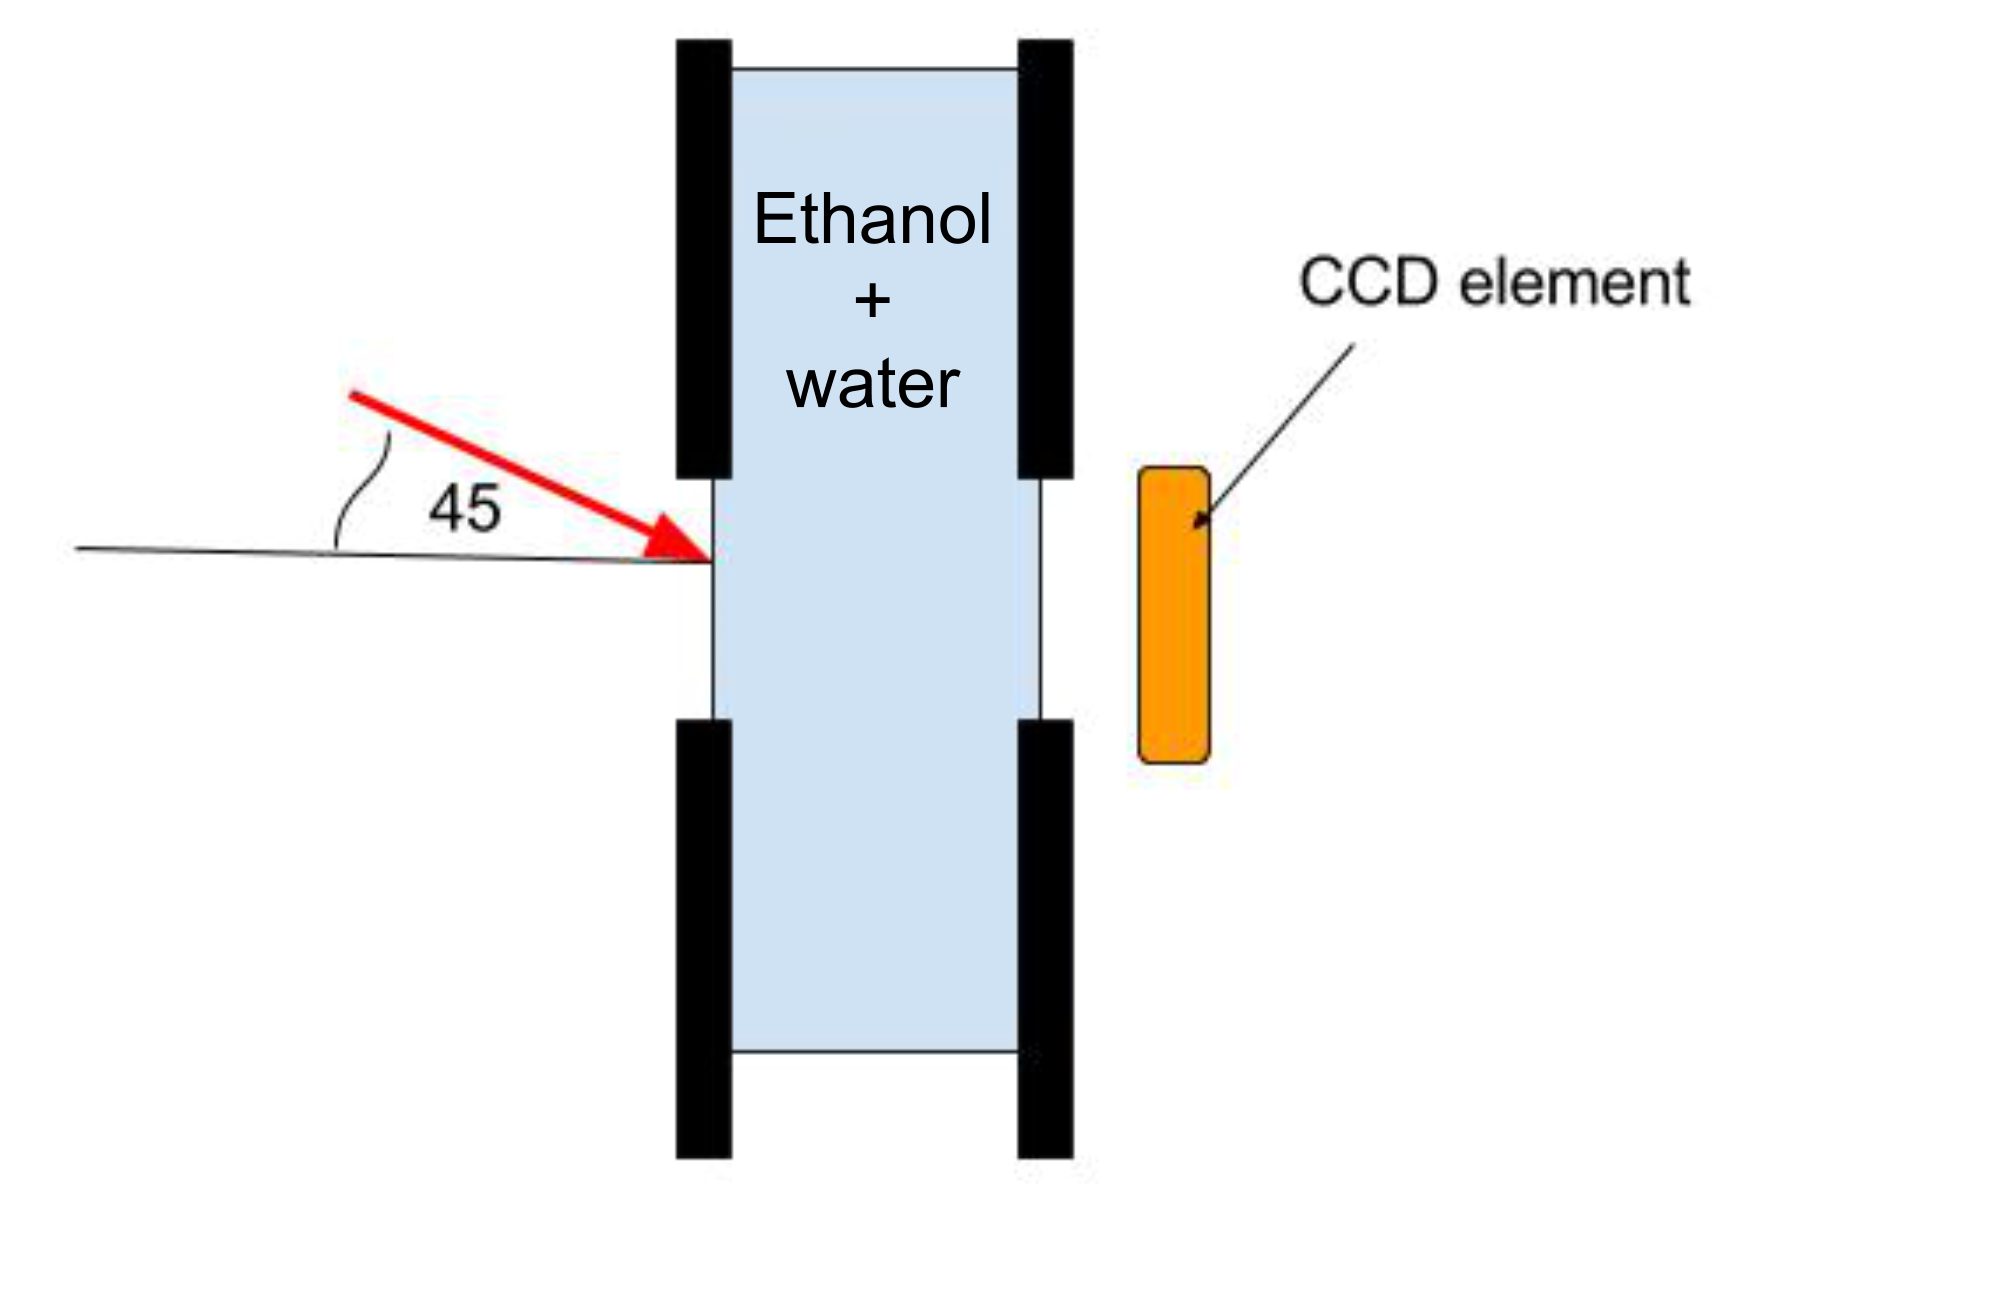
\includegraphics[width=0.5\linewidth]{2017-v2g-04-Piiritusetehas_ing}
	\vspace{-10pt}
\end{center}

\hinteng
The only change in the ray’s trajectory happens in the mixture. Because of the change in the refractive index the ray starts to move at a different angle in the mixture. The according change of angle together with the consequent $y$-directional displacement can be found by using the Snell's law.

\solueng
According to the Snell’s law the following applies during the refraction of light:
$$n_0\sin(\alpha_0)=n_1\sin(\alpha_1),$$ 
where $n_0$ and $n_1$ are respectively the refractive indexes of the first and second environment and $\alpha_0$ and $\alpha_1$ are respectively the angle of incidence and angle of refraction. This formula can be iteratively continued for a next refraction at the border of a third environment where the environments are positioned as parallel layers:
$$n_0\sin(\alpha_0)=n_1\sin(\alpha_1)=n_2\sin(\alpha_2) = \dots$$ 
With this we see that $\sin(\alpha_j)=\frac{n_0}{n_j}\sin(\alpha_0)$ applies. This means that the angle of a ray’s refraction only depends on the environment’s refractive index at this moment and not how many different layers have been previously covered. Because of this we can ignore the layer surrounding the canal that is made of glass or another material and we can calculate the angle of the ray in the canal. In addition, because only the refractive index of the ethanol and the water mixture changes then the angles of movement are different only in the canal. Elsewhere the movement of a ray is exactly the same only that if the refractive index of the mixture is changed then after going through the mixture the ray has been displaced. In the mixture the following applies:
$$\sin(\alpha_{\text{mix}})=\frac{n_0}{n_{\text{mix}}}\sin{\alpha_0} = \frac{1}{\sqrt{2}n_{\text{mix}}},$$ 
where $\sin(\alpha_0) = 1/\sqrt{2}$ and in the air $n_0=1$. With the help of simple geometry the displacement of a ray in the canal along the direction of the canal is 
$$y=d\tan(\alpha_{\text{mix}}).$$ 
Using the relation $\tan(\phi) = \frac{\sin(\phi)}{\cos(\phi)} = \frac{\sin(\phi)}{\sqrt{1-\sin(\phi)^2}}$ we get 
$$y = d \frac{\sin(\alpha_{\text{mix}})}{\sqrt{1-\sin(\alpha_{\text{mix}})^2}} = \frac{d}{\sqrt{2}\sqrt{n_{\text{mix}}^2-\frac12}}.$$ 
Now we find $y$ for two cases: if $X=\num{0.40}$ then $y=\SI{6.184}{\milli\meter}$ and if $X=\num{0.85}$ then $y=\SI{6.104}{\milli\meter}$. We get the difference of $y$ to be
$$|\Delta y| \approx \SI{80}{\micro\meter}.$$
\probend